\documentclass[11pt, letterpaper]{article}
\usepackage[utf8]{inputenc}
\usepackage[margin=1in]{geometry}
\usepackage{enumitem}
\usepackage{indentfirst}
\usepackage{titling}
\usepackage{graphicx}
\usepackage{amsmath}
\usepackage{mathtools}
\usepackage{hyperref}
\usepackage{mathabx}
\usepackage{caption}
\usepackage{subcaption}
\graphicspath{ {./} }
\DeclareMathAlphabet{\altmathcal}{OMS}{cmsy}{m}{n}

\setlength{\parindent}{0cm}
\setlength{\parskip}{1em}
\renewcommand{\baselinestretch}{1.5}

\hypersetup{
    colorlinks=true,
    linkcolor=cyan,
    filecolor=magenta,      
    urlcolor=blue,
}

\title{Chapter IV: Gauss's Law}
\author{Chenyi Zhu}
\date{Feb 4th, 2020}

\begin{document}


\begin{titlingpage}
	\maketitle
	
	\begin{figure}[h!]
		\centering
		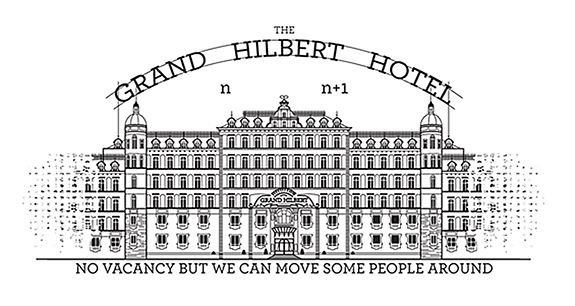
\includegraphics[scale=0.6]{cover}
		\label{fig:flux}
	\end{figure}
		
\end{titlingpage}
	
	\section{Electric Flux.}
	Earlier we discussed the strength of the electric field based on the density of the field lines.
	Now, let us quantify this strength by defining ``electric flux'': the number of field lines passing 
	through any given surface, denoted by $\Phi_E$. Electric field can therefore be considered as
	number of field lines per unit area.
	\begin{figure}[h!]
		\centering
		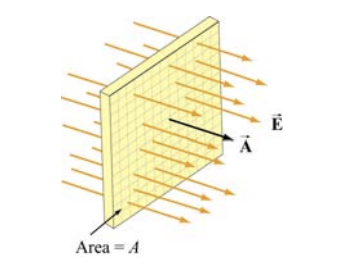
\includegraphics[scale=0.8]{flux}
		\caption{Electric field lines through tilted plane.}
	\end{figure}
	
	We define the area vector $\vec{A} = A\hat{n}$, which has a magnitude the area of the 
	whole surface $A$, and pointing in the normal direction, $\hat{n}$. Place the surface in
	the uniform electric field $\vec{E}$ that points in the same direction as $\hat{n}$, the 
	flux would be:\[\Phi_E = \vec{E}\cdot\vec{A} = \vec{E}\cdot\hat{n}A = EA\]
	and if the electric field $\vec{E}$ makes an angle $\theta$ with $\hat{n}$, the electric
	flux becomes:
	\begin{equation}
		\boxed{\Phi_E = \vec{E}\cdot\vec{A}=EA\cos\theta = E_nA}
	\end{equation}
	and $\theta$ is the angle between the electric field vectors and the normal vector $\hat{n}$
	component of the area vector.\\
	\textbf{Note}: With our definition of the normal vector $\hat{n}$, $\Phi_E$ will be positive
	if electric field lines are leaving the surface, negative if entering the surface.
	
	In a lot of cases, the surface may be curved as opposed to flat. We will be interested in a 
	surface that is \textit{closed}: that the surface completely encloses the volume and there
	are no ``holes''. In this case, we compute the electric flux starting with a little piece of the
	surface $\Delta\vec{A}_i$:
	\begin{figure}
		\centering
		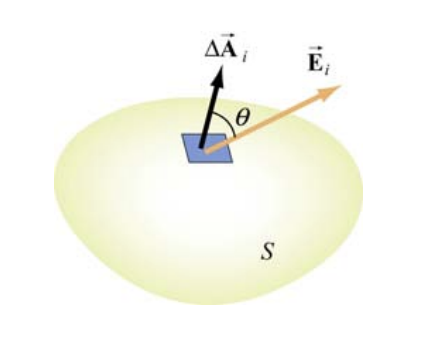
\includegraphics[scale=0.6]{bean}
		\caption{$\vec{E}$ passing through $\Delta\vec{A}_i$ making angle $\theta$ with $\hat{n}$.}
	\end{figure}
	
	\textbf{Note}: The normal unit vector $\hat{n}$ is chosen to point in the outward normal
	direction. 
	
	The flux through $\Delta\vec{A}_i$ is: \[\Delta \Phi_E = \vec{E}_i\cdot\Delta\vec{A}_i = E_i
	\Delta A_i\cos\theta\] and as $\Delta\vec{A}_i \to 0$ and the number of small surface elements
	$\to \infty$:
	\begin{equation}
		\boxed{\Phi_E = \lim_{\Delta \vec{A}_i \to 0}\sum\vec{E}_i\cdot\, d\vec{A}_i = \oiint_S\vec{E}
		\cdot\, d\vec{A}}
	\end{equation}
	where $\oiint_S$ denotes a double integral over a closed surface $S$.
	
	\section{Gauss's Law.}
	Imagine that we have a point charge of $q$, which produces an electric field of $\vec{E} = 
	\frac{Q}{4\pi\varepsilon_0r^2}\,\hat{r}$, pointing radially outwards. We can enclose the
	charge with an imaginary sphere centered at $q$, with radius $r$. We call this sphere the
	``Gaussian surface''.\\
	\textbf{Note}: Here we choose a sphere instead of a cylinder or any other geometries 
	because the field lines coming out of the point charge exhibits spherical symmetry. 
	\begin{figure}[h!]
		\centering
		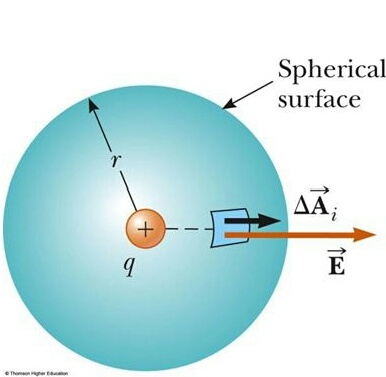
\includegraphics[scale=0.3]{sphere}
		\caption{Point charge and its spherical Gaussian surface.}
	\end{figure}
	
	and in spherical coordinates, a small surface area element on the sphere is given by:
	\[d\vec{A} = r^2\sin\theta d\theta\, d\phi\, \hat{r}\] illustrated by this diagram below:
	\begin{figure}[h!]
		\centering
		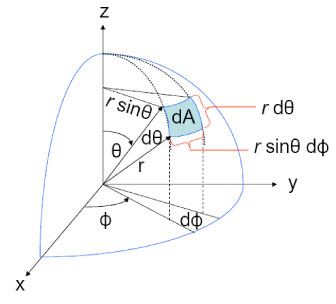
\includegraphics[scale=0.5]{sphere-dA}
		\caption{Representation of small area element on sphere.}
	\end{figure}
	
	We hereby calculate the flux through $d\vec{A}$: \[d\Phi_E=\vec{E}\cdot d\vec{A} = E\, dA
	= \left( \frac{1}{4\pi\varepsilon_0}\frac{q}{r^2}\right)(r^2\sin\theta d\theta\, d\phi) = 
	\frac{q}{4\pi\varepsilon_0}\sin\theta d\theta\, d\phi\] and integration over the entire surface
	will give us:\[\Phi_E = \oiint_S \vec{E}\cdot\, d\vec{A} = E\oiint_S dA = EA = \left( \frac{1}{4\pi
	\varepsilon_0}\frac{q}{r^2}\right)4\pi r^2 = \frac{q}{\varepsilon_0} \]
	
	In this example, we chose a sphere to enclose the point charge because it was the easiest
	to compute mathematically. However, we could technically have chosen any surface (as long
	as it encloses the point charge). 
	
	\textbf{Gauss's Law}:  the net flux through any closed surface is proportional to the net 
	charge enclosed. Mathematically, it is expressed as:
	\begin{equation}
		\boxed{\Phi_E = \oiint_S\vec{E}\cdot\, d\vec{A} = \frac{q_{enc}}{\varepsilon_0}}
	\end{equation}
	See \hyperlink{subsection.4.2}{Appendix} for proof.
	
	In summary, Gauss's law is a convenient tool for evaluating the electric field. \textbf{However},
	its application is only limited to systems that possess certain symmetry (cylindrical, planar,
	and spherical). The table below provides some examples:
	\begin{table}[h!]
	\centering
	\begin{tabular}{||c | c | c||}
	\hline
	\textbf{Symmetry} & 	\textbf{System} & \textbf{Gaussian Surface}\\
	\hline\hline
	Cylindrical & Infinite rod & Coaxial cylinder\\
	\hline
	Planar & Infinite plane & Infinite Box\\
	\hline
	Spherical & Sphere, spherical shell & Concentric sphere\\ \hline
	
	
	\end{tabular}		
	\caption{\label{tab:geometries}Examples of symmetries and corresponding Gaussian
	surfaces.}
	
	\end{table}
	
	\subsection{General Strategies}
	\begin{itemize}
		\item Identify the symmetry exhibited by the system;
		\item Determine the direction of the electric field produced by the system, and then 
		choose the appropriate Gaussian surface such that the electric field would be 
		constant over portions of the surface that we are interested in;
		\item Break down the system into components (e.g. in the pillbox example) and calculate
		$q_{enc}$;
		\item Calculate $\Phi_E$ for each component;
		\item Establish equivalence with Gauss's Law.
		\item See table \hyperlink{subsection.4.1}{here}.
	\end{itemize}
	
	\subsection{Examples}
	\textbf{Example 1}. Infinite rod of charge density $\lambda$.
	
	\textbf{Example 2}. Spherical shell of charge density $\sigma$ and radius $R$.
	
	
	\pagebreak
	
	\section{Conductors.}
	So far, we have seen solid spheres with uniform charge distribution throughout their volume.
	Because of this property, they are called \textbf{insulators}. However, there is another type of
	materials, called \textbf{conductors}, in which electrons can move freely (as opposed to fixed
	in an insulator). Here are the basic properties of a conductor:
	\begin{itemize}
		\item Inside a conductor, $\vec{E} = \vec{0}$. If placed in electric field $\vec{E}_0$, the
		electrons inside will move around to create its own field $\vec{E}'$ to counteract the outer
		field. At equilibrium, inside the conductor, the net electric field $\vec{E} = \vec{E}_0 + 
		\vec{E}'$.
		\item Any net charge must stay on the surface. Let's say we apply charge to a conductor, 
		then it is going to have a net charge. However, the charge will not spread through its
		volume as would inside an insulator, because in that case, $\vec{E} \neq \vec{0}$ according
		to Gauss's Law. Therefore, excess charge remain on the surface.
		\item The tangential component of $\vec{E}$ is $\vec{0}$ on the surface of a conductor.
		\begin{figure}[h!]
			\centering
			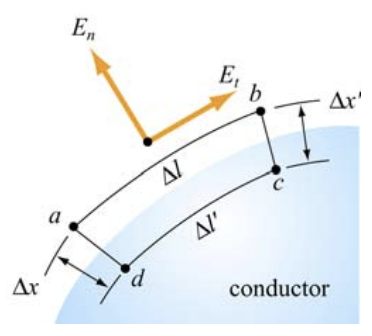
\includegraphics[scale=0.6]{tangent}
			\caption{Surface of a conductor.}
		\end{figure}\\
		Electric field $\vec{E}$ is conservative, therefore the line integral around the closed 
		path $abcda$ must vanish: \[\oint_{abcda}\vec{E}\cdot\, d\vec{s} = E_t(\Delta l) - E_n(\Delta
		x') - 0(\Delta l') + E_n(\Delta x) = 0\] If we take $\Delta x, \, \Delta x' \to 0$ (to approach the
		surface closely), only $E_t(\Delta l)$ remains. And because $\Delta l$ cannot necessarily 
		approach 0, we know that $E_t$ must vanish:
		\begin{equation}
			\boxed{E_t = 0\, \text{(on the surface of the conductor)}}
		\end{equation}
		which implies that the surface of a conductor in electrostatic equilibrium is an 
		\textit{equipotential surface}:\[V_B - V_A = -\int_A^B\vec{E}\cdot\, d\vec{s} = 0\] moving from 
		point $A$ to $B$ on the conductor's surface, because the dot product of two perpendicular 
		vectors is 0.
		\item $\vec{E}$ is normal to the surface just outside the conductor. As with the previous point,
		we saw that only $\vec{E}_n$ survived. Hence, apply Gauss's Law to a charged sheet we
		obtain:\[\Phi_E = \oiint_S\vec{E}\cdot\, d\vec{A} = E_nA = \frac{\sigma A}{\varepsilon_0} 
		\implies \boxed{E_n = \frac{\sigma}{\varepsilon_0}}\] and this result holds for conductors
		with any arbitrary shape.
	\end{itemize}
	
	\pagebreak	
	
	\section{Appendix.}
	\label{Appendix}
	
	\subsection{General Strategies}
	\begin{figure}[h!]
		\centering
		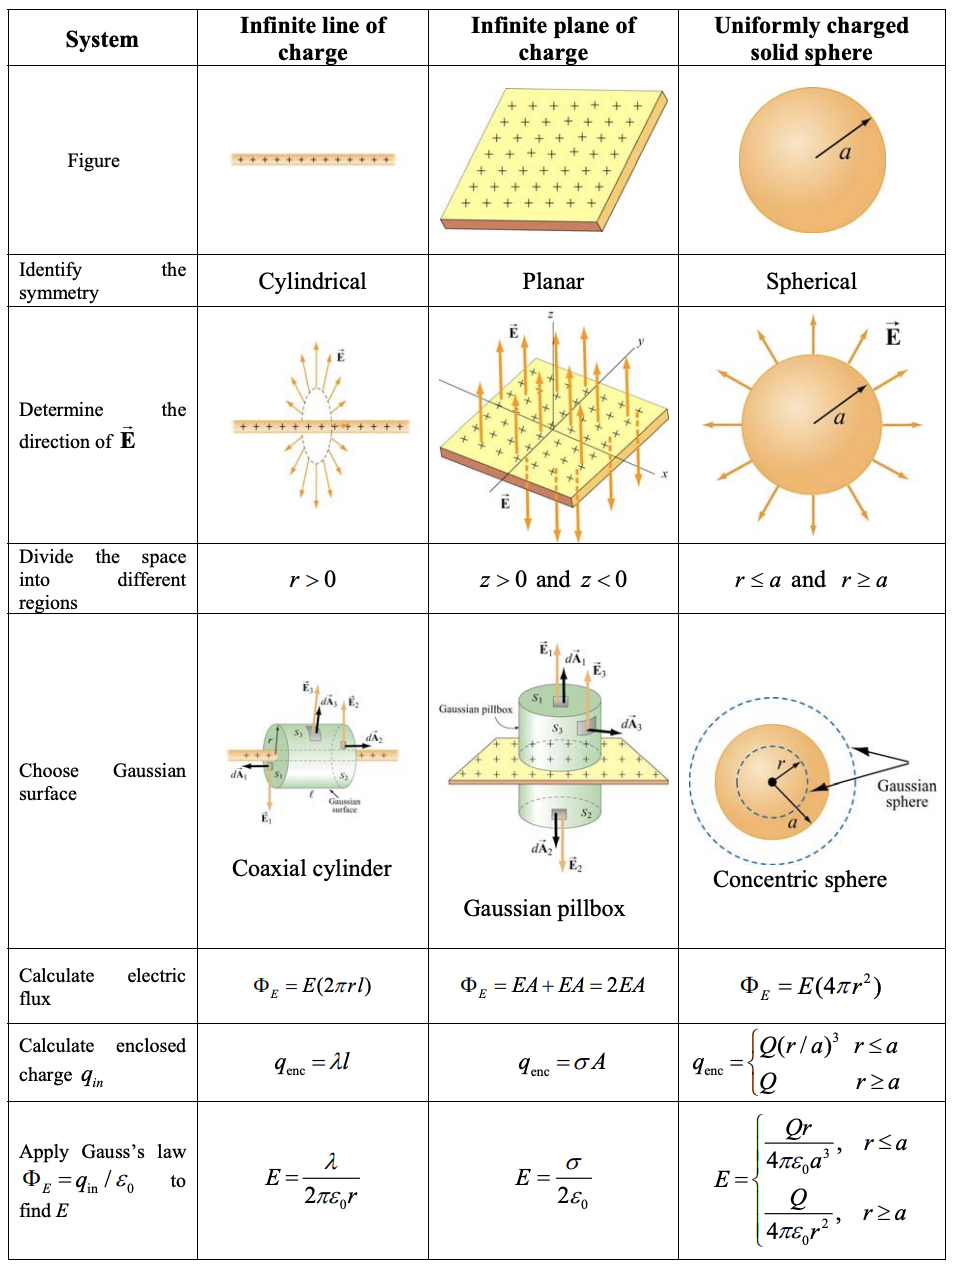
\includegraphics[scale=0.8]{gaussian_guide}
		\caption{General workflow when working with Gaussian surfaces.}
	
	\end{figure}
	
	\subsection{Proof of Gauss's Law}
	In order to prove Gauss's Law, we introduce the concept of a \textbf{solid angle}. Let 
	$\Delta \vec{A}_1 = \Delta A_1\, \hat{r}$ be an area element on the smaller Gaussian sphere 
	$S_1$ of radius $r_1$.
	\begin{figure}[h!]
		\centering
		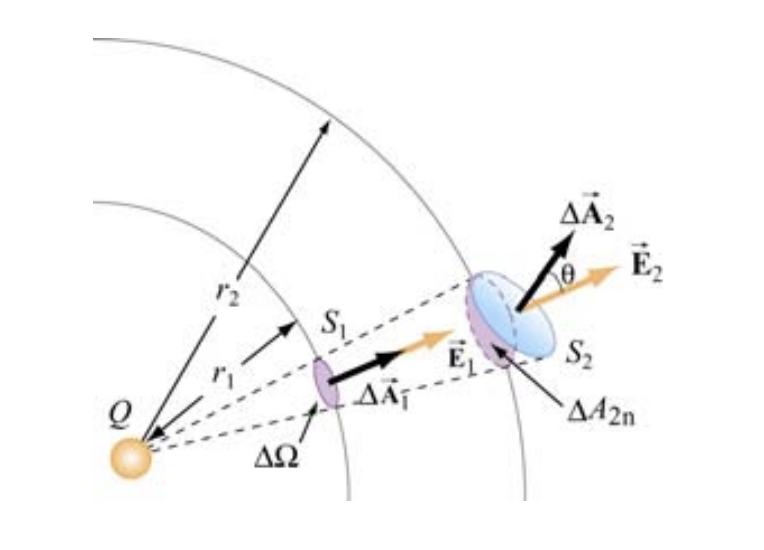
\includegraphics[scale=0.5]{solid_angle}
		\caption{Area element $\Delta A$ subtends a solid angle $\Delta\Omega$.}
	\end{figure}
	
	The solid angle $\Delta \Omega$ subtended by $\Delta \vec{A}_1 = \Delta A_1 \hat{r}$ at the
	center is defined as: \[\Delta \Omega \equiv \frac{\Delta A_1}{r_1^2}\] Just like normal angles,
	solid angles are dimensionless and measured by ``steradians'' (sr). Since the surface area of
	this sphere is $4\pi r_1^2$, we have the total solid angle subtended by the entire sphere as:
	\[\Omega = \frac{4\pi r_1^2}{r_1^2} = 4\pi\]
	Make the connection between solid angles and regular angles!
	
	In the figure we also have a second, bigger Gaussian sphere $S_2$ with radius $r_2$. The
	small area element $\Delta \vec{A}_2$ makes an angle $\theta$ with the radial unit vector 
	$\vec{r}$, then the solid angle subtended by $\Delta A_2$ is: \[\Delta\Omega = 
	\frac{\Delta\vec{A}_2\cdot\hat{r}}{r_2^2} = \frac{\Delta A_2\,\cos\theta}{r_2^2} = \frac{\Delta 
	A_{2n}}{r_2^2}\] Note, now, that the solid angle subtended by both $\Delta A_1$ and 
	$\Delta A_2$ are the same based on the figure above, which gives: \[\frac{\Delta A_1}{
	\Delta A_{2n}} = \frac{r_1^2}{r_2^2}\]
	
	Now suppose that we have a point charge $Q$ a the center of the two concentric spheres.
	The electric field strengths for $S_1$ and $S_2$ are related by Coulomb's Law:
	\[E_i = \frac{1}{4\pi\varepsilon_0}\frac{Q}{r_i^2} \implies \frac{E_2}{E_1} = \frac{r_1^2}{r_2^2}\]
	The electric flux through $\Delta A_1$ is:\[\Delta \Phi_1 = \vec{E}\cdot\Delta \vec{A}_1 = 
	E\Delta A_1\] and the electric flux through $\Delta A_2$ is:\[\Delta\Phi_2 = \vec{E}_2
	\cdot d\vec{A_2} = E\Delta A_2\cos\theta = \left[E_1\left(\frac{r_1^2}{r_2^2}\right)\right]\cdot\left[
	\left(\frac{r_2^2}{r_1^2}\right)\Delta A_1\right] = E_1\Delta A_1 =\Delta\Phi_1\] Thus, without loss
	of generality, we have proved that the electric flux through any surface area element subtending
	the same solid angle is constant, independent of the shape or orientation of the surface.
	
	
	\section{Exercises.}
	%4.8.2
	\subsection{Warm-up}
	\textbf{Problem 1}. Compute the electric flux a) through a square surface of edges $2l$ due to 
	charge $+Q$ located at a perpendicular distance $l$ from the center of the square; b) using the
	results from a), if charge $+Q$ is at the center of a cube of side length $2l$, what is the total
	flux emerging from all six sides of the closed surface?
	\begin{figure}[h!]
		\centering 
		\begin{subfigure}[b]{0.3\textwidth}
			\centering
			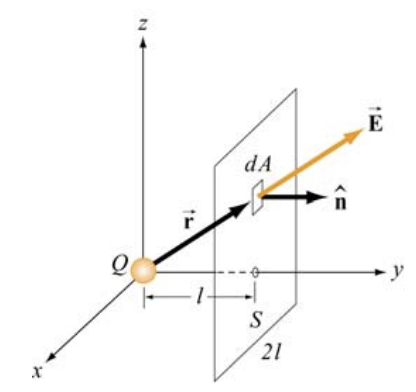
\includegraphics[width=\textwidth]{plane}
			\caption{Electric flux through a plane.}
		\end{subfigure}
		\hspace{2cm}
		\begin{subfigure}[b]{0.3\textwidth}
	    		\centering
			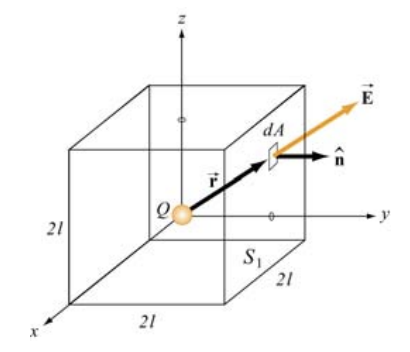
\includegraphics[width=\textwidth]{cube}
			\caption{Electric flux through a cube.}
		\end{subfigure}
	\end{figure}
	
	%4.9.2 & 3
	\subsection{Conceptual Questions}
	\textbf{Problem 2}. Consider the electric field due to a non-conducting infinite plane having a 
	uniform charge density. Why is the electric field independent of the distance from the plane?
	Explain in terms of the spacing of the electric field lines.
	
	\textbf{Problem 3}. If we place a point charge inside a hollow sealed conducting pipe, describe 
	the electric field outside the pipe.
	
	\subsection{More Practice}
	\textbf{Problem 4}. A sphere of radius $2R$ is made of a non-conducting material that has a
	uniform volume charge density $\rho$ (Assume that the material does not affect the electric
	field). A spherical cavity of radius $R$ is then carved out from the sphere, as shown in the figure
    below. Compute the electric field within the cavity.
    \begin{figure}[h!]
    		\centering
    		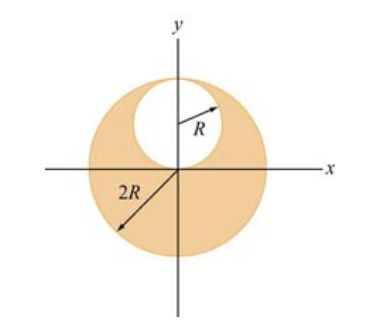
\includegraphics[scale=1]{hollow}
    		\caption{Hole inside non-conducting solid sphere.}
    \end{figure}
    
	\textbf{Problem 5}. What is the gravitational field inside a spherical shell of radius $R$ and mass
	$m$?
	
	
	
	
	
	


\end{document}
